%important---今年：突出了AI；点明了必须要有的部分；不超过15页。
\section{Design of our HPC System}
This section introduces the design of the AI and HPC cluster system.
It begins with an overview of the HPC system architecture, followed by detailed discussions of hardware configuration, software configuration and the interconnection architecture.
Then, we do a comprehensive performance analysis for the computing performance and power consumption.

\subsection{Architectural Diagram Overview}%c-1
\

The HPC cluster design we proposed is shown in Figure \ref{fig:HPCDesign}.
This system adopts a dual-network design with management and data separated, consisting of 4 heterogeneous computing nodes. 
It not only meets the requirements of the competition benchmark but also ensures the high availability of the system. 
\begin{enumerate}
    \item \textbf{Access and Out-of-Band Management: }External users connect to the gigabit Ethernet switch via workstations and utilize the IPMI 2.0 protocol (the blue solid line in the figure) to achieve bottom-level monitoring and out-of-band management of the entire cluster hardware. 
    It supports remote scheduling, power on/off operations, and sensor status monitoring. 
    \item \textbf{Cluster scheduling logic:} Node 0 is configured as the master node (``Master Node"), and cluster management is achieved through a gigabit CAT6 link (indicated by the dotted line in the figure). 
    Its core functions include job scheduling, task distribution, compilation environment hosting, and maintenance of the NFS shared file system. 
    \item \textbf{High-speed interconnection architecture:} The system computing network adopts NDR InfiniBand interconnection (the black solid lines in the figure), and each node is connected to the NDR-IB switch through high-performance HCA cards, providing extremely high throughput bandwidth and microsecond-level latency. 
    \item \textbf{Heterogeneous computing unit}: Each node is constructed based on a dual-processor server and is connected via the PCIe bus to two AMD Radeon Pro W7900D graphics cards. 
    The entire cluster is equipped with a total of 8 high-performance GPUs. 
    With outstanding single/double precision floating-point computing capabilities, it precisely meets the requirements of complex HPC simulations and large-scale AI application.
\end{enumerate}




% Please add the following required packages to your document preamble:
% \usepackage{subfig}
\begin{figure}[!htb]
    \centering
    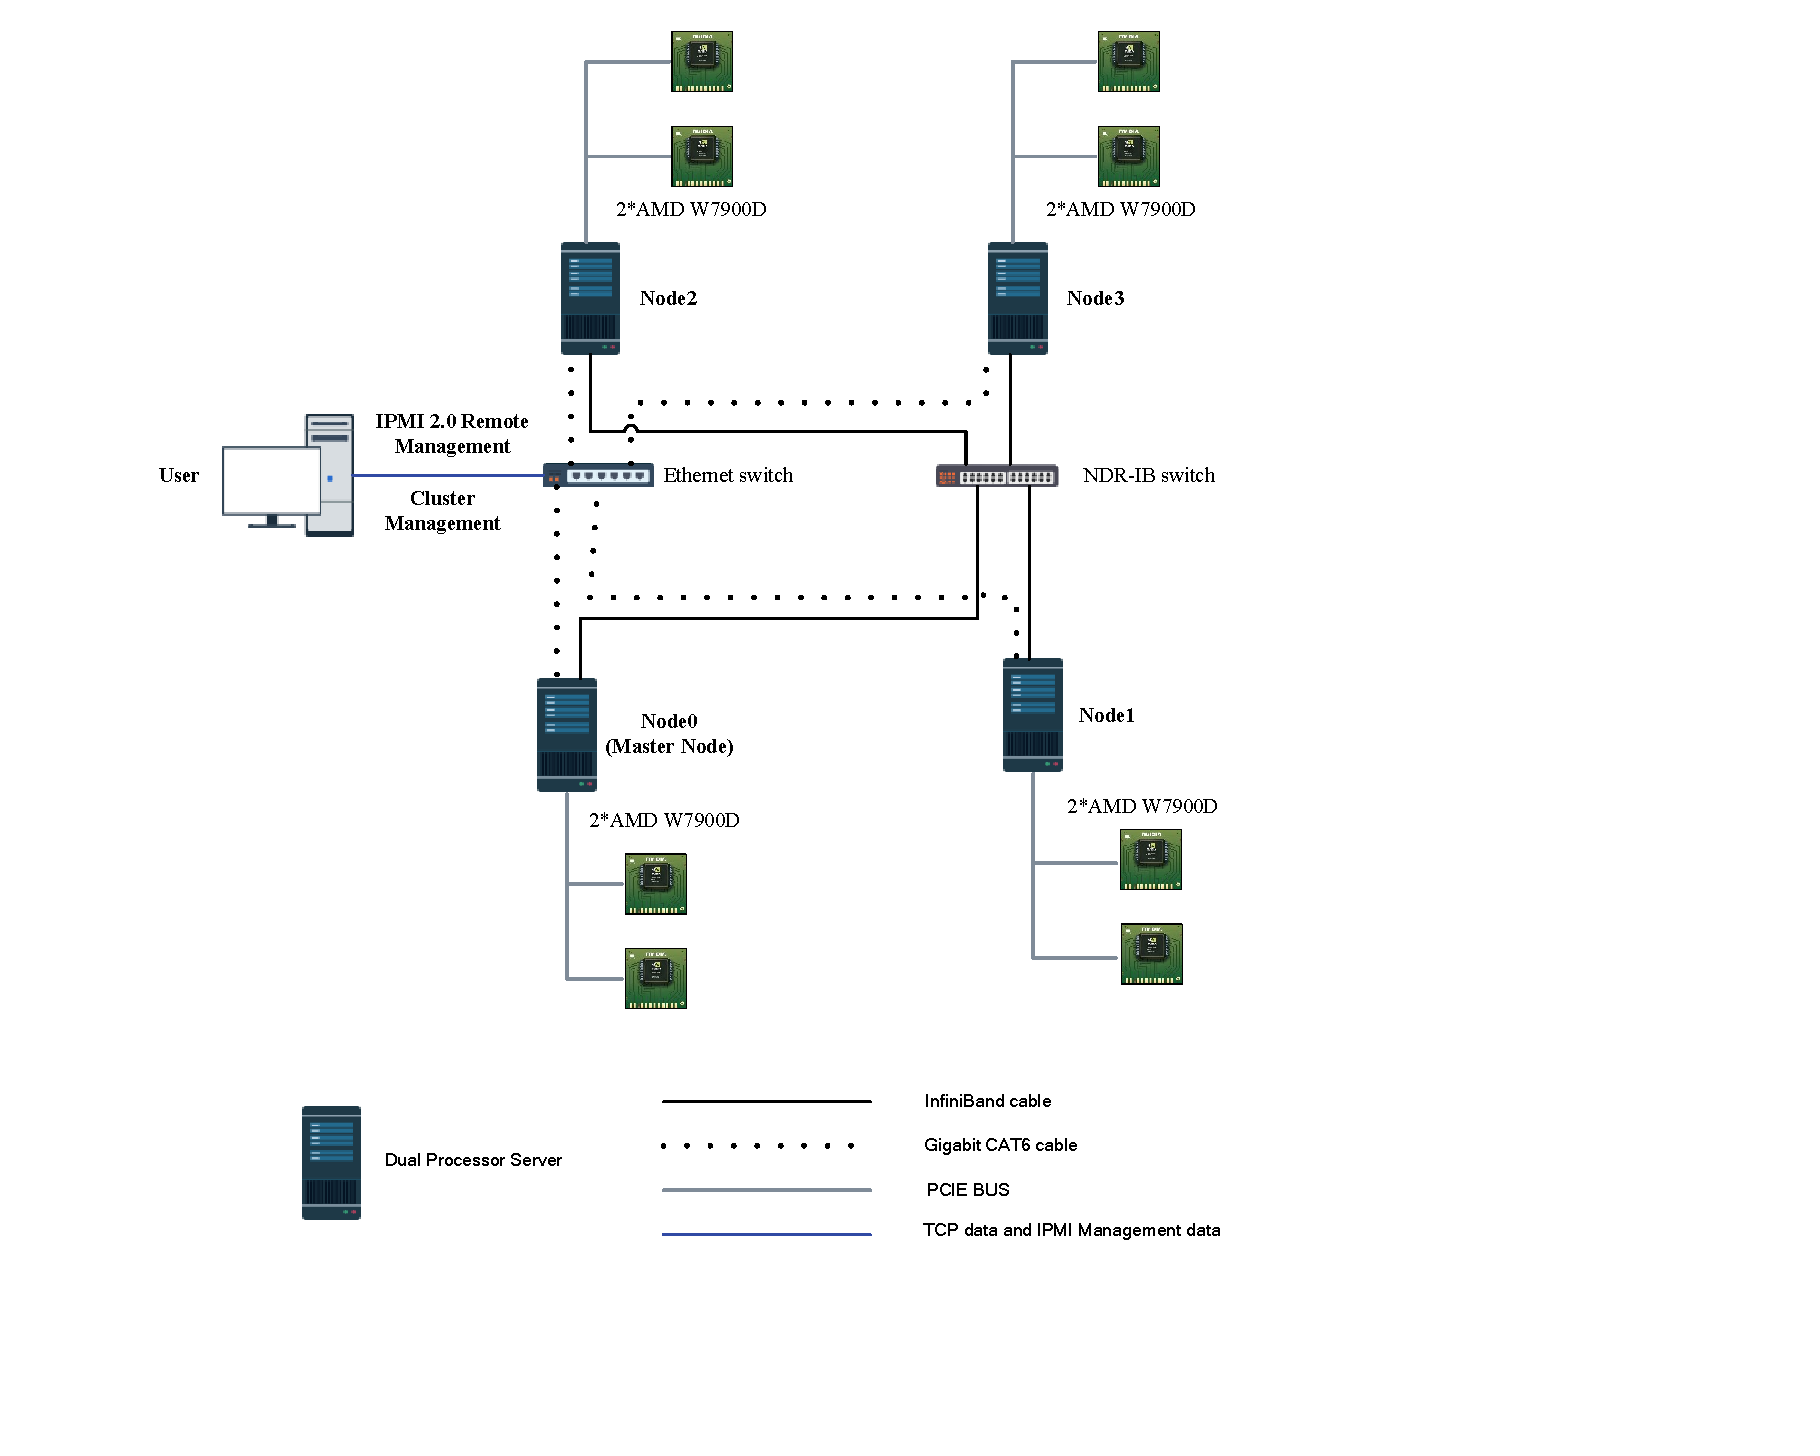
\includegraphics[width=0.98\linewidth]{figures/hpcDesign-0221.pdf}
    \caption{Architectural Diagram Overview}
    \label{fig:HPCDesign}
\end{figure}


\subsection{System Configuration and Architecture Analysis}%b
\


\subsubsection{Hardware Configurations}
\


The complete technical specifications of the designed HPC system are systematically presented in Table \ref{tab:hpc hardware}.
This high-performance computing system is a small heterogeneous computing cluster, which is a cost-effective and balanced heterogeneous workstation cluster. 
Although its local storage I/O speed is slightly conservative, its powerful interconnection capability and computing density enable it to fully handle the ASC supercomputing competition and complex AI research tasks. 
The detailed analysis is as follows. 
Firstly, in terms of CPU processors, each computing node is equipped with two processors recommended by the committee, namely AMD EPYC 9755 with the latest Zen 5 architecture, each with 128 cores and 512M cache. 
The entire cluster has a total of 1024 physical cores, and it has strong capabilities in multi-threaded tasks and instruction-level parallelism (ILP). 
Secondly, at the accelerator (GPU) level, the entire cluster is equipped with 8 AMD Radeon Pro W7900D workstation graphics cards, with 2 cards per node. 
The W7900D is based on the RDNA 3 architecture, with a huge memory capacity and high bandwidth, making it a powerful tool for AI inference and graphics rendering.
In the storage and memory level, each node is configured with 768GB DDR5 memory ($32GB \times 24$), with a clock speed of up to 6400 MT/s, ensuring a large bandwidth to meet the data feeding requirements of a multi-core CPU. 
The system disk uses a 960GB SATA SSD, balancing startup speed and stability. 
Finally, the high-speed network uses the NVIDIA Quantum-2 NDR InfiniBand switch, providing a single port throughput of 400Gbps, and combined with the MCX75310AAS-NEAT HCA card, it achieves extremely low one-way latency.

\begin{table}[h]
\centering
\caption{Hardware resources details}
\label{tab:hpc hardware}
\renewcommand{\arraystretch}{1.2} % 增加行间距，使表格更美观
\begin{tabular}{|c|l|c|}
\hline
\rowcolor{myyellow}
\textbf{Item} & \multicolumn{1}{c|}{\textbf{Name}} & \textbf{Quantity} \\ \hline
 & CPU: AMD 9755-EPYC 2.7\_128C\_512M * 2 & 4 \\ \cline{2-3} 
 & Memory: 32GB * 24, DDR5, 6400 MT/s & 4 \\ \cline{2-3} 
 & Hard disk: 960GB SSD SATA * 1 & 4 \\ \cline{2-3} 
\multirow{-4}{*}{Dual Processor Server} & Motherboard Power Consumption & 4 \\ \hline
GPU & AMD W7900D & 8 \\ \hline
HCA & NDR400: NVIDIA MCX75310AAS-NEAT & 4 \\ \hline
 & Ethernet switch: 10/100/1000 MB/s, 24 ports Ethernet switch & 1 \\ \cline{2-3} 
\multirow{-2}{*}{Switch} & \begin{tabular}[c]{@{}l@{}}NDR-IB switch: NVIDIA Quantum (TM)-2 NDR InfiniBand Switch\\ , 64-ports NDR, 32 OSFP ports, unmanaged, P2C airflow (forward)\end{tabular} & 1 \\ \hline
 & Gigabit CAT6 cables & 5 \\ \cline{2-3} 
\multirow{-2}{*}{Cable} & InfiniBand cable & 4 \\ \hline
\end{tabular}
\end{table}

\subsubsection{Software Configurations}
\

Since the CPU and GPU of this HPC system are both sourced from AMD, in order to enable the system to run large-scale computing and artificial intelligence operations efficiently, its main software configuration follows the AMD recommended configuration\footnote{https://www.amd.com/en/developer.html}. 
The details are shown in Table \ref{tab:hpc software}. 
The operating system selected is Ubuntu 24.04 LTS as the underlying operating system. 
As the latest long-term support version, it can provide excellent stability and compatibility for high-performance hardware. 
For GPU heterogeneous computing, the latest stable version ROCm 7.2 is configured, providing complete support from the underlying driver to the high-level library, including MIOpen (deep learning primitive library) and rocBLAS (linear algebra library). 
For the CPU system deployment, Zen Software Studio 2.0 is configured, whose core includes AOCC (a compiler highly optimized for the Zen 5 architecture), AOCL (an optimized math library), ZenDNN (an inference acceleration library), and AMD uProf (a performance analysis tool). 
At the application layer, Anaconda is used to build an isolated and repeatable scientific computing environment, with the latest versions of PyTorch, TensorFlow, and JAX, etc. integrated.



\begin{table}[h]
\centering
\caption{Software resources details}
\label{tab:hpc software}
\renewcommand{\arraystretch}{1.2} % 增加行间距，使表格更美观
\begin{tabular}{|C{4cm}|L{10cm}|C{2cm}|}
\hline
\rowcolor{myyellow}
\textbf{Item} & \textbf{Name} & \textbf{Version} \\ \hline
Application software & Anaconda(including PyTorch, TensorFlow, JAX and so on) & Version 2.3 \\ \hline
GPU & ROCm  & Version 7.2 \\ \hline
CPU & AMD Zen Software Studio(including AMD uProf, AOCL, AOCC, ZenDNN and so on) & Version 2.0 \\ \hline
Operating system & Ubuntu & 24.04 LTS \\ \hline
\end{tabular}
\end{table}



\subsubsection{Interconnection Architecture}
\

As shown in the Figure \ref{fig:HPCDesign}, the HPC system of this design adopts a ``management network + data network" separated architecture and uses a star topology. 
The ``Master Node" serves as the cluster entry point and is mainly responsible for task distribution management. 
The compute nodes are mainly responsible for computing. 
Low-latency data exchange is achieved through InfiniBand, and remote IPMI and cluster control are realized through Ethernet.

\subsection{Computing Performance Description}
\

Based on the relevant parameters of AMD 9755-EPYC \footnote{https://www.amd.com/en/products/processors/server/epyc/9005-series/amd-epyc-9755.html}
and AMD Radeon Pro W7900D\footnote{https://www.amd.com/en/products/graphics/workstations/radeon-pro/w7900.html}, the performance analysis of the CPU and GPU for our HPC system is as follows.

The peak performance calculation formula for the CPU is 
\begin{equation}
         \text{Peak Performance} = \text{Clock Speed} \times \text{Cores} \times \text{Operations per Cycle}.
\end{equation}

\begin{enumerate}
    \item \textbf{Clock speed: }Since the ``Base clock" of AMD 9755-EPYC is 2.7GHz and the ``Max. Boost Clock" is 4.1GHz, here we will calculate its highest computing performance. 
    Therefore, we set the clock speed to 4.1GHz.
    \item \textbf{Cores: }HPC consists of 4 computing nodes, and each computing node contains 2 CPUs with 128 cores. 
    Therefore, the cores included in HPC are $4{\times}2{\times}128{=}1024$.
    \item \textbf{Operations per Cycle: }In the competition, if floating-point operations use single-precision floating-point numbers, then since the Zen 5 architecture has a complete 512-bit (512-bit) vector unit, each 512-bit register can store 8 FP64 numbers. 
    Also, since the CPU supports FMA (Fused Multiply-Add) instructions (2 FMA units), one cycle can complete one multiplication and one addition (counted as 2 operations). 
    Therefore, the single-cycle operation count of AMD 9755-EPYC can be $2{\times}8{\times}2{=}32 flops/Cycle$.
\end{enumerate}  

Based on the above information, the final peak CPU performance of the HPC is
\begin{equation}
         4.1GHz{\times}1024(Cores){\times}32 (\text{Operations per Cycle})\\
          =134.3488TLOPs
\end{equation}


According to the official website information, the peak double float precision(FP64), single float precision (FP32 Vector)  and half float precision(FP16) performance of the AMD Radeon Pro W7900D single GPU are 1.916 Tflops, 61.3 Tflops and 123 Tflops, respectively.
And there are a total of 8 GPUs in the cluster. 
Therefore, the overall theoretical peak performance of the GPUs is based on different precisions are as follows.
\begin{equation}
    \text{FP64 Peak Performance} {=} 1.916 TLOPs \times 8 {=} 15.328 TLOPs.
\end{equation}

\begin{equation}
    \text{FP32 Peak Performance} {=} 61.3 TLOPs \times 8 {=} 490.4 TLOPs.
\end{equation}

\begin{equation}
    \text{FP16 Peak Performance} {=} 123 TLOPs \times 8 {=} 984 TLOPs.
\end{equation}



\subsection{Power Consumption Description}%c-2
\


Our HPC cluster comprises four computing nodes. 
This section provides a detailed analysis of power consumption patterns for both GPU and CPU operations at individual node level and cluster-wide scale, as detailed in Table \ref{tab:power}. 
As can be seen from the table, for a single node, the CPU computing power consumption is $1054W{+}40W{=}1094W$, and the GPU computing power consumption is $354W{+}2×295W{=}944W$, both of which meet the power consumption requirement of less than $2000W$. 
For the entire cluster, the CPU computing power consumption is
$4926W$, and the GPU computing power consumption is $4326W$, which also meet the power consumption requirement of less than $5000W$.




\begin{table}[htbp]
\centering
\small
\caption{Power Consumption Details}
\label{tab:power}
\begin{tabular}{|C{1.8cm}|C{2.5cm}|L{7.5cm}|C{1.8cm}|}
\hline
\rowcolor{myyellow}
\textbf{Mode} & \textbf{Name} & \multicolumn{2}{|c|}{\arraybackslash\textbf{Power Consumption}} \tabularnewline
\hline
\multirow{11}{=}{CPU computing} 
 & \multirow{4}{=}{Dual Processor Server} 
   & CPU: AMD 9755-EPYC2.7 128C 512M * 2 (450w * 2) 
   & \multirow{4}{*}{1054w*4} \tabularnewline
\cline{3-3}
 &  & Memory: 32GB * 24, DDR5, 6400 MT/s (5w * 24) &  \tabularnewline
\cline{3-3}
 &  & Hard disk: 960GB SSD SATA * 1 (4w * 1) &  \tabularnewline
\cline{3-3}
 &  & Motherboard Power Consumption (30w) &  \tabularnewline
\cline{2-4}
 & GPU & AMD W7900D & 20w*8 \tabularnewline
\cline{2-4}
 & HCA & NDR400: NVIDIA MCX75310AAS-NEAT & 30w*4 \tabularnewline
\cline{2-4}
 & \multirow{2}{*}{Switch} 
   & Ethernet switch: 10/100/1000 MB/s, 24 ports Ethernet switch 
   & 30w \tabularnewline
\cline{3-4}
 &  & NDR-IB switch: NVIDIA Quantum (TM)-2 NDR InfiniBand Switch, 64-ports 
   & 400w \tabularnewline
\cline{2-4}
 & \multicolumn{2}{c|}{\textbf{Total}} & \textbf{4926w} \tabularnewline
\hline
\multirow{11}{=}{GPU computing} 
 & \multirow{4}{=}{Dual Processor Server} 
   & CPU: AMD 9755-EPYC2.7 128C 512M * 2 (100w * 2) 
   & \multirow{4}{*}{354w*4} \tabularnewline
\cline{3-3}
 &  & Memory: 32GB * 24, DDR5, 6400 MT/s (5w * 24) &  \tabularnewline
\cline{3-3}
 &  & Hard disk: 960GB SSD SATA * 1 (4w * 1) &  \tabularnewline
\cline{3-3}
 &  & Motherboard Power Consumption (30w) &  \tabularnewline
\cline{2-4}
 & GPU & AMD W7900D (295w) & 295w*8 \tabularnewline
\cline{2-4}
 & HCA & NDR400: NVIDIA MCX75310AAS-NEAT & 30w*4 \tabularnewline
\cline{2-4}
 & \multirow{2}{*}{Switch} 
   & Ethernet switch: 10/100/1000 MB/s, 24 ports Ethernet switch 
   & 30w \tabularnewline
\cline{3-4}
 &  & NDR-IB switch: NVIDIA Quantum (TM)-2 NDR InfiniBand Switch, 64-ports 
   & 400w \tabularnewline
\cline{2-4}
 & \multicolumn{2}{c|}{\textbf{Total}} & \textbf{4326w} \tabularnewline
\hline
\end{tabular}
\end{table}



